\documentclass{article}
\usepackage{fullpage,amsmath,amsthm,graphicx,enumitem,amsfonts}
\usepackage{multicol}
\usepackage{booktabs}

\usepackage{tikz}

\theoremstyle{definition}
\newtheorem{thm}{Theorem}
\newtheorem{question}[thm]{Question}
\newenvironment{solution}{\noindent\textit{Solution:}}{}

\title{ASEN 5264 Decision Making under Uncertainty\\
       Quiz 1: Probabilistic Models and MDPs}

\date{\small Clearly indicate your final answers and briefly justify numerical answers with text or mathematical expressions.\\
If you do not understand how to do a problem, skip it and move on so that you have time to attempt all problems.\\
You may consult any static source, but you may NOT communicate with any person except the instructor or TA, and you may not use LLMs such as ChatGPT.}

\begin{document}
\maketitle

\begin{question} (30 pts)
    Consider the following Bayesian network made up of binary random variables:
    \begin{center}
    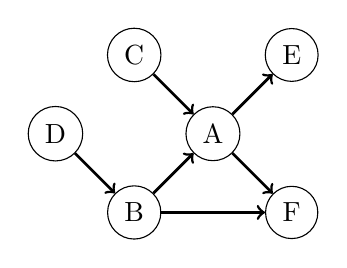
\begin{tikzpicture}
        \node[shape=circle,draw=black] (D) at (0,0) {D};
        \node[shape=circle,draw=black] (A) at (2,0) {A};
        \node[shape=circle,draw=black] (C) at (1,1) {C};
        \node[shape=circle,draw=black] (E) at (3,1) {E};
        \node[shape=circle,draw=black] (F) at (3,-1) {F};
        \node[shape=circle,draw=black] (B) at (1,-1) {B};
        \path [->,line width=1pt] (B) edge node[left]{}(A);
        \path [->,line width=1pt] (D) edge node[left]{}(B);
        \path [->,line width=1pt] (C) edge node[left]{}(A);
        \path [->,line width=1pt] (A) edge node[left]{}(F);
        \path [->,line width=1pt] (A) edge node[left]{}(E);
        \path [->,line width=1pt] (B) edge node[left]{}(F);
    \end{tikzpicture}
    \end{center}

    \begin{enumerate}[label=\alph*)]
        \item Is it possible to conclude from the structure only that $E \perp C \mid A$?
        \item Is it possible to conclude from the structure only that $F \perp C \mid A$?
        \item Suppose $P(E=1 \mid A=1) = 0.8$. Find $P(E=0 \mid A=1, C=1)$ if possible with the given information.
        \item Suppose $P(E=1 \mid A=1) = 0.8$. Find $P(E=1 \mid A=0, C=1)$ if possible with the given information.
        \item Suppose $P(F=1 \mid A=1) = 0.7$. Find $P(F=0 \mid A=1, C=1)$ if possible with the given information.
    \end{enumerate}
\end{question}

\clearpage

\begin{question} (30 pts)
    Consider the following one player game. During the game, you will flip two fair coins, one after the other. Before the first flip, your friend guesses the outcome, heads or tails. If your friend guesses correctly on the first flip, you pay her \$2. Before the second flip, your friend again guesses heads or tails, but this time you pay her \$1 for each coin that has landed that way. For example if she guesses heads on the second step and both coins were heads, you again pay her \$2.

    Formulate this as a Markov decision process from your friend's perspective by writing down the state space, action space, transition probabilities, reward function, and discount factor. Recall that the reward function can be expressed as $R(s, a, s')$.
\end{question}
%     Consider the following one player game. You flip a fair coin twice in succession. Before each flip, your friend tries to guess the number the total number of heads that will have occurred after the flip. After each flip, if your friend has guessed correctly, you pay her \$2. If she guesses incorrectly, she pays you \$1. Formulate this as a Markov decision process from your friend's perspective by writing down the state space, action space, transition probabilities, reward function, and discount factor. Recall that the reward function can be expressed as $R(s, a, s')$.



\clearpage

\begin{question} (30 pts)
    Consider the following MDP: $S = A = \{1,2\}$, $R(s, a) = \begin{cases}
            2 & \text{if } s = a\\
            -1 & \text{otherwise}
        \end{cases}$, $\gamma = 0.9$.

        If the action is odd, there is a 90\% chance of transitioning to the odd state. If the action is even, there is an 80\% chance of transitioning to the even state. Suppose that you are performing policy iteration and have computed the value function for the current policy $\pi$ as $U^\pi = \begin{bmatrix}
            1 \\
            5
            \end{bmatrix}$.
    \begin{enumerate}[label=\alph*)]
        \item Perform the policy update/improvement step of policy iteration to find a new policy $\pi'$.
        \item Give a matrix equation for the value of the new policy $\pi'$. Fill in numbers in all vectors and matrices except $U^{\pi'}$, but you do not need to solve the equation.
    \end{enumerate}
\end{question}

\clearpage

\begin{question} (10 pts)
    Suppose that a 21 state MDP has state space consisting of consecutive integers, $S = \{-10, -9, \ldots, 9, 10\}$, action space $\{-1, 1\}$, reward function $R(s, a)=s^2$, and discount $\gamma=0.96$. I claim to have an optimal policy $\pi$ that achieves an expected  cumulative discounted reward of 2500 if the initial state is 1, that is $U^\pi(1) = 2500$. Is it possible to prove or disprove my claim with the given information? Explain.
\end{question}

\end{document}
